\subsection{Peking}

Comencemos por describir la ruta generada(Ver mapa que todavía no está). Se han realizado 29 saltos hasta alcanzar el destino solicitado, de los cuales en el $86 \% $ de los mismos aproximadamente, hemos obtenido respuestas del tipo $TIME\_EXCEEDED$, determinando, así que el largo de nuestra ruta es de 25 saltos, y que del resto de los valores del $TTL$ no hemos obtenido respuesta alguna. Como también se puede ver en el (mapa que no está), durante el trayecto se realizaron 3 saltos intercontinentales, en los ttls 6, 10 Y 20. Por otro lado, el método de Cimbala nos ha detectado todo número positivo como outlier en primera instancia y al sacar los 0s nos devolvió como outliers los ttls 6, 10, 12, 14, 15, 20, 21.


Al realizar el experimento, se logró llegar al destino en el ttl 29. De estos, 4 no respondieron. Los ttls que Cimbala reconoció como intercontinentales fueron 6, 10, 12, 14, 15, 20, 21.

\begin{figure}[!htbp]
  \centering
    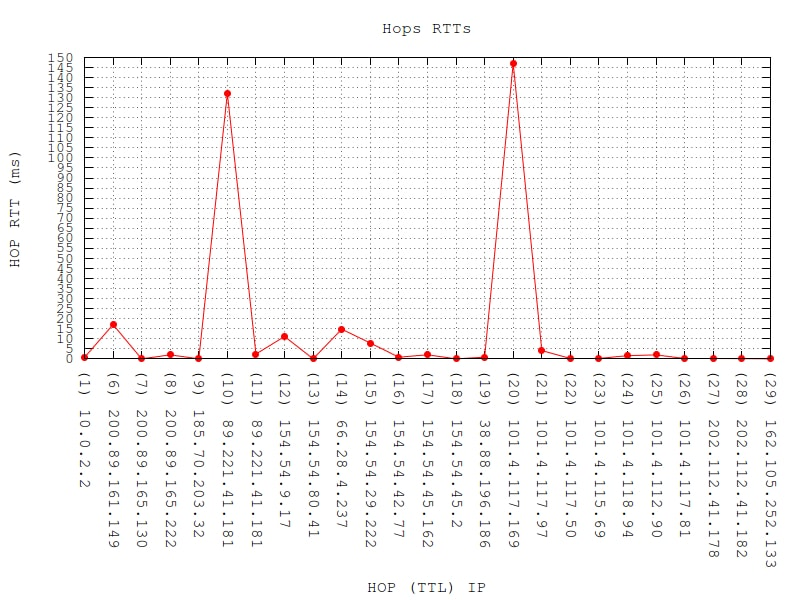
\includegraphics[scale=0.6]{imagenes/peking-graficos/traceroute-peking.jpg}
  \caption{peking- RTT hops}
  \label{fig:10}
\end{figure}

En la figura \ref{fig:10} se puede observar como el ttl 10 y 20 tienen un rtt claramente distinguido del resto.

\begin{figure}[!htbp]
  \centering
    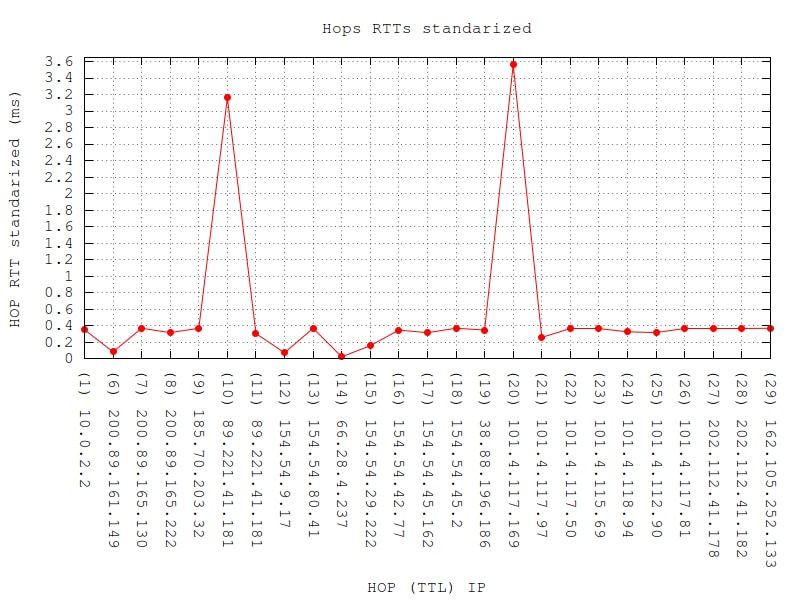
\includegraphics[scale=0.6]{imagenes/peking-graficos/traceroute-peking-standarized.jpg}
  \caption{peking- RTT hops standarized}
  \label{fig:11}
\end{figure}

En la figura \ref{fig:11} se puede observar una situacion similar a la de la figura \ref{fig:10}.

